\documentclass[14pt]{extbook}
\usepackage{multicol, enumerate, enumitem, hyperref, color, soul, setspace, parskip, fancyhdr} %General Packages
\usepackage{amssymb, amsthm, amsmath, latexsym, units, mathtools} %Math Packages
\everymath{\displaystyle} %All math in Display Style
% Packages with additional options
\usepackage[headsep=0.5cm,headheight=12pt, left=1 in,right= 1 in,top= 1 in,bottom= 1 in]{geometry}
\usepackage[usenames,dvipsnames]{xcolor}
\usepackage{dashrule}  % Package to use the command below to create lines between items
\newcommand{\litem}[1]{\item#1\hspace*{-1cm}\rule{\textwidth}{0.4pt}}
\pagestyle{fancy}
\lhead{Makeup Progress Quiz 3}
\chead{}
\rhead{Version ALL}
\lfoot{1648-1753}
\cfoot{}
\rfoot{Summer C 2021}
\begin{document}

\begin{enumerate}
\litem{
For the graph below, find the value(s) $a$ that makes the statement true: $ \displaystyle \lim_{x \rightarrow a} f(x)$ does not exist.
\begin{center}
    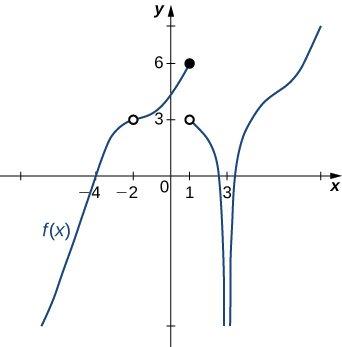
\includegraphics[width=0.5\textwidth]{../Figures/evaluateLimitGraphicallyCopyA.png}
\end{center}
\begin{enumerate}[label=\Alph*.]
\item \( -2 \)
\item \( 1 \)
\item \( 3 \)
\item \( \text{Multiple } a \text{ make the statement true}. \)
\item \( \text{No } a \text{ make the statement true}. \)

\end{enumerate} }
\litem{
Evaluate the one-sided limit of the function $f(x)$ below, if possible.\[ \lim_{x \rightarrow 7^+} \frac{-5}{(x+7)^4}+7 \]\begin{enumerate}[label=\Alph*.]
\item \( \infty \)
\item \( f(7) \)
\item \( -\infty \)
\item \( \text{The limit does not exist} \)
\item \( \text{None of the above} \)

\end{enumerate} }
\litem{
Evaluate the limit below, if possible.\[ \lim_{x \rightarrow 8} \frac{\sqrt{7x - 7} - 7}{5x - 40} \]\begin{enumerate}[label=\Alph*.]
\item \( 0.071 \)
\item \( 0.100 \)
\item \( \infty \)
\item \( 0.014 \)
\item \( \text{None of the above} \)

\end{enumerate} }
\litem{
Evaluate the limit below, if possible.\[ \lim_{x \rightarrow 5} \frac{\sqrt{8x - 4} - 6}{6x - 30} \]\begin{enumerate}[label=\Alph*.]
\item \( \infty \)
\item \( 0.111 \)
\item \( 0.083 \)
\item \( 0.471 \)
\item \( \text{None of the above} \)

\end{enumerate} }
\litem{
Based on the information below, which of the following statements is always true?
\begin{center}
    \textit{ $f(x)$ approaches $17.923$ as $x$ approaches $7$. }
\end{center}
\begin{enumerate}[label=\Alph*.]
\item \( f(17) \text{ is close to or exactly } 7 \)
\item \( f(7) = 17 \)
\item \( f(7) \text{ is close to or exactly } 17 \)
\item \( f(17) = 7 \)
\item \( \text{None of the above are always true.} \)

\end{enumerate} }
\litem{
For the graph below, evaluate the limit: $ \displaystyle \lim_{x \rightarrow -4} f(x)$.
\begin{center}
    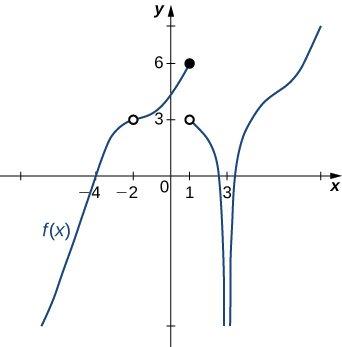
\includegraphics[width=0.5\textwidth]{../Figures/evaluateLimitGraphicallyA.png}
\end{center}
\begin{enumerate}[label=\Alph*.]
\item \( -6 \)
\item \( 0 \)
\item \( -\infty \)
\item \( \text{The limit does not exist} \)
\item \( \text{None of the above} \)

\end{enumerate} }
\litem{
Evaluate the one-sided limit of the function $f(x)$ below, if possible.\[ \lim_{x \rightarrow 1^-} \frac{7}{(x+1)^7}+8 \]\begin{enumerate}[label=\Alph*.]
\item \( f(1) \)
\item \( \infty \)
\item \( -\infty \)
\item \( \text{The limit does not exist} \)
\item \( \text{None of the above} \)

\end{enumerate} }
\litem{
Based on the information below, which of the following statements is always true?
\begin{center}
    \textit{ As $x$ approaches $\infty$, $f(x)$ approaches $9.495$. }
\end{center}
\begin{enumerate}[label=\Alph*.]
\item \( f(x) \text{ is close to or exactly } 9.495 \text{ when } x \text{ is large enough}. \)
\item \( f(x) \text{ is undefined when } x \text{ is large enough}. \)
\item \( f(x) \text{ is close to or exactly } \infty \text{ when } x \text{ is large enough}. \)
\item \( x \text{ is undefined when } f(x) \text{ is large enough}. \)
\item \( \text{None of the above are always true.} \)

\end{enumerate} }
\litem{
To estimate the one-sided limit of the function below as $x$ approaches 4 from the left, which of the following sets of numbers should you use?\[ \frac{\frac{4}{x} - 1}{x - 4} \]\begin{enumerate}[label=\Alph*.]
\item \( \{ 4.0000, 3.9000, 3.9900, 3.9990 \} \)
\item \( \{ 3.9000, 3.9900, 4.0100, 4.1000 \} \)
\item \( \{ 4.0000, 4.1000, 4.0100, 4.0010 \} \)
\item \( \{ 3.9000, 3.9900, 3.9990, 3.9999 \} \)
\item \( \{ 4.1000, 4.0100, 4.0010, 4.0001 \} \)

\end{enumerate} }
\litem{
To estimate the one-sided limit of the function below as $x$ approaches 4 from the right, which of the following sets of numbers should you use?\[ \frac{\frac{4}{x} - 1}{x - 4} \]\begin{enumerate}[label=\Alph*.]
\item \( \{ 4.1000, 4.0100, 4.0010, 4.0001 \} \)
\item \( \{ 3.9000, 3.9900, 4.0100, 4.1000 \} \)
\item \( \{ 4.0000, 3.9000, 3.9900, 3.9990 \} \)
\item \( \{ 4.0000, 4.1000, 4.0100, 4.0010 \} \)
\item \( \{ 3.9000, 3.9900, 3.9990, 3.9999 \} \)

\end{enumerate} }
\litem{
For the graph below, find the value(s) $a$ that makes the statement true: $ \displaystyle \lim_{x \rightarrow a} f(x)$ does not exist.
\begin{center}
    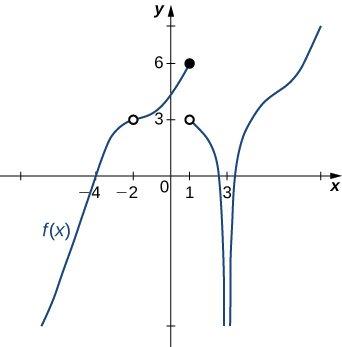
\includegraphics[width=0.5\textwidth]{../Figures/evaluateLimitGraphicallyCopyB.png}
\end{center}
\begin{enumerate}[label=\Alph*.]
\item \( -2 \)
\item \( 1 \)
\item \( 3 \)
\item \( \text{Multiple } a \text{ make the statement true}. \)
\item \( \text{No } a \text{ make the statement true}. \)

\end{enumerate} }
\litem{
Evaluate the one-sided limit of the function $f(x)$ below, if possible.\[ \lim_{x \rightarrow 8^+} \frac{-4}{(x+8)^4}+6 \]\begin{enumerate}[label=\Alph*.]
\item \( \infty \)
\item \( f(8) \)
\item \( -\infty \)
\item \( \text{The limit does not exist} \)
\item \( \text{None of the above} \)

\end{enumerate} }
\litem{
Evaluate the limit below, if possible.\[ \lim_{x \rightarrow 5} \frac{\sqrt{6x - 14} - 4}{7x - 35} \]\begin{enumerate}[label=\Alph*.]
\item \( \infty \)
\item \( 0.350 \)
\item \( 0.018 \)
\item \( 0.125 \)
\item \( \text{None of the above} \)

\end{enumerate} }
\litem{
Evaluate the limit below, if possible.\[ \lim_{x \rightarrow 6} \frac{\sqrt{6x - 20} - 4}{5x - 30} \]\begin{enumerate}[label=\Alph*.]
\item \( 0.125 \)
\item \( 0.025 \)
\item \( 0.490 \)
\item \( \infty \)
\item \( \text{None of the above} \)

\end{enumerate} }
\litem{
Based on the information below, which of the following statements is always true?
\begin{center}
    \textit{ $f(x)$ approaches $4.192$ as $x$ approaches $1$. }
\end{center}
\begin{enumerate}[label=\Alph*.]
\item \( f(1) \text{ is close to or exactly } 4 \)
\item \( f(4) \text{ is close to or exactly } 1 \)
\item \( f(4) = 1 \)
\item \( f(1) = 4 \)
\item \( \text{None of the above are always true.} \)

\end{enumerate} }
\litem{
For the graph below, find the value(s) $a$ that makes the statement true: $ \displaystyle \lim_{x \rightarrow a} f(x)$ does not exist.
\begin{center}
    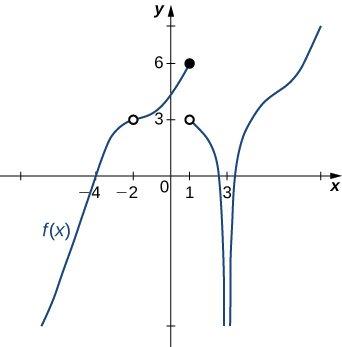
\includegraphics[width=0.5\textwidth]{../Figures/evaluateLimitGraphicallyB.png}
\end{center}
\begin{enumerate}[label=\Alph*.]
\item \( 3 \)
\item \( 1 \)
\item \( -2 \)
\item \( \text{Multiple } a \text{ make the statement true}. \)
\item \( \text{No } a \text{ make the statement true}. \)

\end{enumerate} }
\litem{
Evaluate the one-sided limit of the function $f(x)$ below, if possible.\[ \lim_{x \rightarrow -1^+} \frac{6}{(x+1)^4}+7 \]\begin{enumerate}[label=\Alph*.]
\item \( f(-1) \)
\item \( -\infty \)
\item \( \infty \)
\item \( \text{The limit does not exist} \)
\item \( \text{None of the above} \)

\end{enumerate} }
\litem{
Based on the information below, which of the following statements is always true?
\begin{center}
    \textit{ As $x$ approaches $0$, $f(x)$ approaches $15.316$. }
\end{center}
\begin{enumerate}[label=\Alph*.]
\item \( f(x) \text{ is close to or exactly } 0 \text{ when } x \text{ is close to } 15.316 \)
\item \( f(x) = 0 \text{ when } x \text{ is close to } 15.316 \)
\item \( f(x) \text{ is close to or exactly } 15.316 \text{ when } x \text{ is close to } 0 \)
\item \( f(x) = 15.316 \text{ when } x \text{ is close to } 0 \)
\item \( \text{None of the above are always true.} \)

\end{enumerate} }
\litem{
To estimate the one-sided limit of the function below as $x$ approaches 5 from the right, which of the following sets of numbers should you use?\[ \frac{\frac{5}{x} - 1}{x - 5} \]\begin{enumerate}[label=\Alph*.]
\item \( \{ 4.9000, 4.9900, 4.9990, 4.9999 \} \)
\item \( \{ 5.0000, 5.1000, 5.0100, 5.0010 \} \)
\item \( \{ 5.0000, 4.9000, 4.9900, 4.9990 \} \)
\item \( \{ 4.9000, 4.9900, 5.0100, 5.1000 \} \)
\item \( \{ 5.1000, 5.0100, 5.0010, 5.0001 \} \)

\end{enumerate} }
\litem{
To estimate the one-sided limit of the function below as $x$ approaches 6 from the left, which of the following sets of numbers should you use?\[ \frac{\frac{6}{x} - 1}{x - 6} \]\begin{enumerate}[label=\Alph*.]
\item \( \{ 5.9000, 5.9900, 6.0100, 6.1000 \} \)
\item \( \{ 6.1000, 6.0100, 6.0010, 6.0001 \} \)
\item \( \{ 6.0000, 6.1000, 6.0100, 6.0010 \} \)
\item \( \{ 6.0000, 5.9000, 5.9900, 5.9990 \} \)
\item \( \{ 5.9000, 5.9900, 5.9990, 5.9999 \} \)

\end{enumerate} }
\litem{
For the graph below, find the value(s) $a$ that makes the statement true: $ \displaystyle \lim_{x \rightarrow a} f(x)$ does not exist.
\begin{center}
    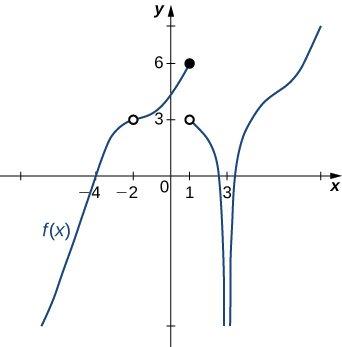
\includegraphics[width=0.5\textwidth]{../Figures/evaluateLimitGraphicallyCopyC.png}
\end{center}
\begin{enumerate}[label=\Alph*.]
\item \( 1 \)
\item \( -2 \)
\item \( 3 \)
\item \( \text{Multiple } a \text{ make the statement true}. \)
\item \( \text{No } a \text{ make the statement true}. \)

\end{enumerate} }
\litem{
Evaluate the one-sided limit of the function $f(x)$ below, if possible.\[ \lim_{x \rightarrow 2^-} \frac{8}{(x+2)^3}+7 \]\begin{enumerate}[label=\Alph*.]
\item \( \infty \)
\item \( f(2) \)
\item \( -\infty \)
\item \( \text{The limit does not exist} \)
\item \( \text{None of the above} \)

\end{enumerate} }
\litem{
Evaluate the limit below, if possible.\[ \lim_{x \rightarrow 5} \frac{\sqrt{9x - 9} - 6}{3x - 15} \]\begin{enumerate}[label=\Alph*.]
\item \( \infty \)
\item \( 0.028 \)
\item \( 0.083 \)
\item \( 1.000 \)
\item \( \text{None of the above} \)

\end{enumerate} }
\litem{
Evaluate the limit below, if possible.\[ \lim_{x \rightarrow 9} \frac{\sqrt{5x - 20} - 5}{9x - 81} \]\begin{enumerate}[label=\Alph*.]
\item \( 0.100 \)
\item \( \infty \)
\item \( 0.248 \)
\item \( 0.056 \)
\item \( \text{None of the above} \)

\end{enumerate} }
\litem{
Based on the information below, which of the following statements is always true?
\begin{center}
    \textit{ As $x$ approaches $7$, $f(x)$ approaches $5.372$. }
\end{center}
\begin{enumerate}[label=\Alph*.]
\item \( f(7) \text{ is close to or exactly } 5 \)
\item \( f(5) = 7 \)
\item \( f(5) \text{ is close to or exactly } 7 \)
\item \( f(7) = 5 \)
\item \( \text{None of the above are always true.} \)

\end{enumerate} }
\litem{
For the graph below, find the value(s) $a$ that makes the statement true: $ \displaystyle \lim_{x \rightarrow a} f(x)$ does not exist.
\begin{center}
    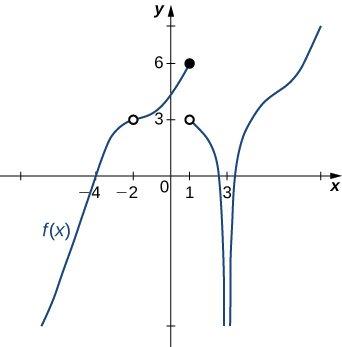
\includegraphics[width=0.5\textwidth]{../Figures/evaluateLimitGraphicallyC.png}
\end{center}
\begin{enumerate}[label=\Alph*.]
\item \( 1 \)
\item \( 3 \)
\item \( -2 \)
\item \( \text{Multiple } a \text{ make the statement true}. \)
\item \( \text{No } a \text{ make the statement true}. \)

\end{enumerate} }
\litem{
Evaluate the one-sided limit of the function $f(x)$ below, if possible.\[ \lim_{x \rightarrow 8^+} \frac{-5}{(x+8)^5}+7 \]\begin{enumerate}[label=\Alph*.]
\item \( -\infty \)
\item \( \infty \)
\item \( f(8) \)
\item \( \text{The limit does not exist} \)
\item \( \text{None of the above} \)

\end{enumerate} }
\litem{
Based on the information below, which of the following statements is always true?
\begin{center}
    \textit{ $f(x)$ approaches $5.4$ as $x$ approaches $2$. }
\end{center}
\begin{enumerate}[label=\Alph*.]
\item \( f(2) \text{ is close to or exactly } 5 \)
\item \( f(5) = 2 \)
\item \( f(5) \text{ is close to or exactly } 2 \)
\item \( f(2) = 5 \)
\item \( \text{None of the above are always true.} \)

\end{enumerate} }
\litem{
To estimate the one-sided limit of the function below as $x$ approaches 7 from the right, which of the following sets of numbers should you use?\[ \frac{\frac{7}{x} - 1}{x - 7} \]\begin{enumerate}[label=\Alph*.]
\item \( \{ 7.1000, 7.0100, 7.0010, 7.0001 \} \)
\item \( \{ 7.0000, 6.9000, 6.9900, 6.9990 \} \)
\item \( \{ 6.9000, 6.9900, 7.0100, 7.1000 \} \)
\item \( \{ 6.9000, 6.9900, 6.9990, 6.9999 \} \)
\item \( \{ 7.0000, 7.1000, 7.0100, 7.0010 \} \)

\end{enumerate} }
\litem{
To estimate the one-sided limit of the function below as $x$ approaches 9 from the left, which of the following sets of numbers should you use?\[ \frac{\frac{9}{x} - 1}{x - 9} \]\begin{enumerate}[label=\Alph*.]
\item \( \{ 9.0000, 9.1000, 9.0100, 9.0010 \} \)
\item \( \{ 9.0000, 8.9000, 8.9900, 8.9990 \} \)
\item \( \{ 8.9000, 8.9900, 8.9990, 8.9999 \} \)
\item \( \{ 9.1000, 9.0100, 9.0010, 9.0001 \} \)
\item \( \{ 8.9000, 8.9900, 9.0100, 9.1000 \} \)

\end{enumerate} }
\end{enumerate}

\end{document}